\documentclass[a4paper]{report}

%====================== PACKAGES ======================

\usepackage[french]{babel}
\usepackage[utf8x]{inputenc}
%pour gérer les positionnement d'images
\usepackage{float}
\usepackage{amsmath}
\usepackage{graphicx}
\usepackage[colorinlistoftodos]{todonotes}
\usepackage{url}
%pour les informations sur un document compilé en PDF et les liens externes / internes
\usepackage{hyperref}
%pour la mise en page des tableaux
\usepackage{array}
\usepackage{tabularx}
%pour utiliser \floatbarrier
%\usepackage{placeins}
%\usepackage{floatrow}
%espacement entre les lignes
\usepackage{setspace}
%modifier la mise en page de l'abstract
\usepackage{abstract}
%police et mise en page (marges) du document
\usepackage[T1]{fontenc}
\usepackage[top=2cm, bottom=2cm, left=2cm, right=2cm]{geometry}
%Pour les galerie d'images
\usepackage{subfig}

%====================== INFORMATION ET REGLES ======================

%rajouter les numérotation pour les \paragraphe et \subparagraphe
\setcounter{secnumdepth}{4}
\setcounter{tocdepth}{4}

\hypersetup{							% Information sur le document
pdfauthor = {Premier Auteur,
			Deuxième Auteur,
			Troisième Auteur,
    		Quatrième Auteur},			% Auteurs
pdftitle = {Nom du Projet -
			Sujet du Projet},			% Titre du document
pdfsubject = {Mémoire de Projet},		% Sujet
pdfkeywords = {Tag1, Tag2, Tag3, ...},	% Mots-clefs
pdfstartview={FitH}}					% ajuste la page à la largueur de l'écran
%pdfcreator = {MikTeX},% Logiciel qui a crée le document
%pdfproducer = {}} % Société avec produit le logiciel

%======================== DEBUT DU DOCUMENT ========================

\begin{document}

%régler l'espacement entre les lignes
\newcommand{\HRule}{\rule{\linewidth}{0.5mm}}

%page de garde
\begin{titlepage}
\begin{center}

% Upper part of the page. The '~' is needed because only works if a paragraph has started.


\includegraphics[width=0.35\textwidth]{./logo}~\\[1cm]

\includegraphics[width=0.35\textwidth]{./omega}~\\[1cm]

%\textsc{\LARGE OmegeSoft-Agadir}\\[1.5cm]


\textsc{\Large }\\[0.5cm]

% Title
\HRule \\[0.4cm]

{\huge \bfseries Contrôle à distance\\
Stage d'apprentissage et de recherche  \\[0.4cm] }

\HRule \\[1.5cm]

% Author and supervisor
\begin{minipage}{0.4\textwidth}
\begin{flushleft} \large
\emph{Auteur:}\\
Yahya \textsc{ETTAHI}\\
%Deuxième \textsc{Auteur}\\
%Troisième \textsc{Auteur}\\
%Quatrième \textsc{Auteur}
\end{flushleft}
\end{minipage}
\begin{minipage}{0.4\textwidth}
\begin{flushright} \large
\emph{Ecadrant:} \\
Dr. Abdelilah \textsc{KAHAJI}\\
%\emph{Référent:} \\
%Prénom \textsc{Nom}
\end{flushright}
\end{minipage}

\vfill

% Bottom of the page
{\large \today}

\end{center}
\end{titlepage}

%page blanche
\newpage
~
%ne pas numéroter cette page
\thispagestyle{empty}
\newpage

\renewcommand{\abstractnamefont}{\normalfont\Large\bfseries}
%\renewcommand{\abstracttextfont}{\normalfont\Huge}

\begin{abstract}
\hskip7mm

\begin{spacing}{1.3}

J’ai réalisé mon stage dans la société OmegaSoft, cette société est une SSII (Société de Services et d'Ingénierie Informatique) spésialisé dans le développement d’application, la formation professionnelle et l’infogérance de services informatiques. Mon rôle consistait à comprendre comment TeamViewer\footnotemark fonctionne, et pourquoi pas trouver un altérnatif du logiciel précédent .
Pour cela, j’ai suit des formations en réseau (en ligne) à titre d'exemple : Reprenez le contrôle à l'aide de Linux \cite{ref1}, Apprenez le fonctionnement des réseaux TCP/IP \cite{ref2}, Prenez le contrôle à distance d'un poste Linux/Windows avec VNC \cite{ref3} .
Ainsi, enrichir mon bagage informatique et améliorer ma capacité de recherche et d'analyse.  



\footnotetext{TeamViewer est un logiciel propriétaire de télémaintenance disposant de fonctions de bureau à distance, de téléadministration, de conférence en ligne et de transfert de fichiers.}


\end{spacing}
\end{abstract}



\tableofcontents
\thispagestyle{empty}
\setcounter{page}{0}
%ne pas numéroter le sommaire

\newpage

%espacement entre les lignes d'un tableau
\renewcommand{\arraystretch}{1.5}

%====================== INCLUSION DES PARTIES ======================

~
\thispagestyle{empty}
%recommencer la numérotation des pages à "1"
\setcounter{page}{0}
\newpage

\chapter{Contexte}


\section{Introduction}

%note en bas de page

La téléadministration, ou prise de contrôle à distance d'un ordinateur et de son système d'exploitation dans le but d’administrer le système (sauvegarde, mises à jour logiciel, etc.) et de résoudre les problèmes applicatifs des utilisateurs, est une solution bien adaptée aux PME \cite{ref4}. \\

Cette maintenance à distance consiste à prendre le contrôle via le réseau local ou Internet. Aujourd'hui, elle peut également être utilisée pour gérer un système d'exploitation virtualisé, hébergé en local ou également à distance. La télémaintenance se fait par le biais d'outils d'administration à distance qui proposent plus ou moins de fonctionnalités, comme le transfert de fichiers par exemple. Certains systèmes, comme KVM ou le port série, nécessitent un appareil connecté à la machine distante et pouvant être contrôlé depuis le poste de travail du technicien de maintenance.

    Les protocoles suivants sont ouverts et ont différentes applications ouvertes ou fermées : Commutateur écran-clavier-souris (ou commutateur KVM, indépendant du système), IPMI (indépendant du système, mais dépendant du matériel), Remote Desktop Protocol (ou RDP, indépendant du système), rsh (Remote Shell), Secure Shell (SSH) (ligne de commande ou export application X11 (ou X Window System), Telnet, XDMCP (X Window System) et VNC (indépendant du système), liaison série (généralement UART) compatible VT100 (console texte, indépendant du système, très utilisé dans les systèmes embarqués).

La plupart des systèmes d'exploitations comportent par défaut un ou plusieurs système de contrôle à distance, comme :

    RDP, telnet pour Microsoft Windows,
    RDP, telnet, rsh, SSH, UART (via TTY) VNC, XDMCP sur Linux ou BSD.

D'autres logiciels ont été développés par des sociétés tierces, permettent la télémaintenance, en passant généralement par des protocoles fermés ou l'un des protocoles ouverts définis ci-dessus : Bomgar, Checklan, NetOp Remote Control, DameWare, Ivanti Endpoint Manager, LogMeIn, PC Anywhere, TeamViewer, Ammyy Admin. 
Bla\\
%saut de paragraphe

Bla

\newpage

\section{Problématique soulevée}

Bla

\begin{center}
Problématique du sujet
\end{center}

\section{Hypothèse de solution}

%Quoi :
Bla\\

Voici une liste :
\begin{itemize}
\item item 1;
\item item 2;
\item item 3;
\item item 4.
\end{itemize}

Bla\\

%Comment :
Bla

Bla\footnotemark\\

%Detail :
Bla(cf. ref. \cite{cite6}).
%citation référencé dans le document "bibliographie.bib" inclus à la fin du document

\footnotetext{Note bas de page "bla"}




\chapter{Problématique}

Intro

\section{Partie 1}

Intro

\subsection{Sous-partie 1}

Bla

\subsection{Sous-partie 2}

Bla\\

Transition

\section{Partie 2}

Bla\\

Transition

\section{Bilan récapitulatif}

Voici un tableau (cf. fig. 2.1) récapitulatif de notre analyse de l'existant...\\

%tableau centré à taille variable qui s'ajuste automatiquement suivant la longueur du contenu
\begin{figure}[!h]
\begin{center}
\begin{tabular}{|l|l|l|l|l|}
  \hline
  Solution & Critère 1 & Critère 2 & Critère 3 & Critère 4\\
  \hline
  Solution 1(cf. ref. \cite{cite0}) & Oui & Oui & Oui & Oui \\
  Solution 2(cf. ref. \cite{cite1}) & Oui & Oui & Oui & Non \\
  Solution 3(cf. ref. \cite{cite2}) & Oui (sauf telle chose) & Non & Non & Oui\\
  Solution 4(cf. ref. \cite{cite3}) & Oui& Non & Oui & Non\\
  Solution 5(cf. ref. \cite{cite4}) & Oui (uniquement ceux-ci) & Non & Oui & Non\\
  \hline
\end{tabular}
\end{center}
\caption{Tableau récapitulatif des solutions}
\end{figure}

 
\chapter{Recherche}

Intro

\section{Besoins fonctionnels}

Après une analyse des besoins fonctionnels du projet, nous avons défini deux sous catégories. D'un côté, les besoins [...], de l'autre, les besoins [...].

\subsection{Sous-partie 1}

Bla

\subsection{Sous-partie 2}

Bla

\newpage

\section{Besoins non-fonctionnels}

Comme précédemment, nous avons choisi de distinguer deux catégories pour les besoins non-fonctionnels. D'une part, nous avons les besoins non-fonctionnels pour les [...], et d'autre part ceux pour [...]. Nous avons aussi pris en compte les contraintes de développement, que nous détaillerons à la fin de cette partie.

\subsection{Sous-partie 1}

Bla\\

Aperçu du rendu souhaité :

\begin{figure}[!h]
\begin{center}
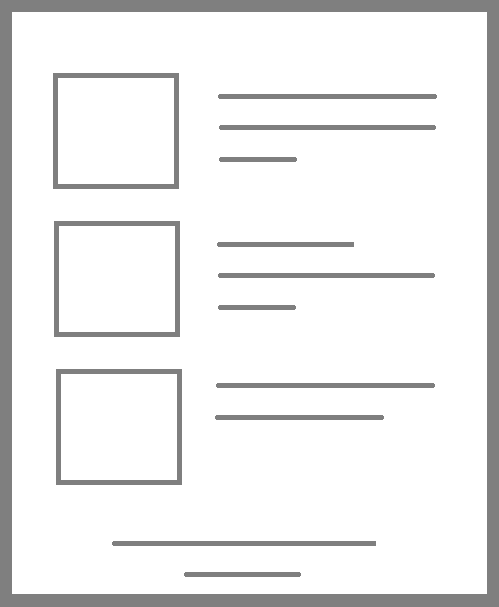
\includegraphics[height=10cm]{besoins/rendu}
\end{center}
\caption{Rendu attendu}
\end{figure}

\subsection{Sous-partie 2}

Bla

\newpage

\section{Développement}

Intro

\subsection{Tâches}

Bla\\


%tableau à taille fixée sur certaines colonnes (param sur la ligne \begin{tabularx}, voir wiki pour plus d'info sur la syntaxe
\begin{figure}[!h]
\begin{center}
\begin{tabularx}{17cm}{|c|p{6cm}|X|}
  \hline
  Priorité & Nom & Raison\\
  \hline
  1 & Tache 1 & Doit être vérifié en premier car sinon [...] \tabularnewline
  2 & Tache 2 & On doit pouvoir [...] \tabularnewline
  3 & Tache 3 & Comme les principales fonctionnalités permettant de tester sont opérationnelles, nous pouvons passer à cette tâche. \tabularnewline
  4 & Tache 4 & Parce que [...] \tabularnewline
  5 & Tache 5 & La tache 5 fait partie des principales [...]. \tabularnewline
  6 & Tache 6 & Dernière fonctionnalité essentielle à mettre en place. \tabularnewline
  7 & Tache 7 & Non-essentiel, mais apporterait un plus au projet. \tabularnewline
  8 & Tache 8 & Non-essentiel, mais apporterait un plus au projet. \tabularnewline
  \hline
\end{tabularx}
\end{center}
\caption{Tableau récapitulatif des tâches}
\end{figure}

\subsection{Tests}

Bla\\

\begin{figure}[!h]
\begin{center}
\begin{tabularx}{17cm}{|p{6cm}|X|}
  \hline
  Fonctionnalité & Test\\
  \hline
  Fonction 1 & Quand [...], vérifier [...]. \tabularnewline
  & Et quand [...], vérifier [...]. \tabularnewline
  Fonction 2 & Vérifier [...]. \tabularnewline
  Fonction 3 & Vérifier [...]. \tabularnewline
  Fonction 4 & Avoir [...]. \tabularnewline
  Fonction 5 & Accéder à [...]. \tabularnewline
   & Vérifier que [...]. \tabularnewline
  Fonction 6 & Accéder à [...]. \tabularnewline
   & Et vérifier [...]. \tabularnewline
  Fonction 7 & Installer [...]. \tabularnewline
   & Vérifier [...]. \tabularnewline
  Fonction 8 & Compter [...]. \tabularnewline
  \hline
\end{tabularx}
\end{center}
\caption{Tableau récapitulatif des tests}
\end{figure}

%\chapter{Résultats}

\section{Partie 1}

Intro

\subsection{Sous-partie 1}

\paragraph*{Paragraphe 1 (n'apparaitra pas dans l'index)} Bla

\paragraph*{Paragraphe 2} Bla

\paragraph*{Paragraphe 3} Bla

\subsection{Sous-partie 2}

Bla

\subsection{Sous-partie 3}

Bla

\section{Partie 2}

Intro

\subsection*{Sous-partie 1 ('apparaitra pas dans l'index)} Bla

\paragraph*{Paragraphe 1 ('apparaitra pas dans l'index)} Bla

\paragraph*{Paragraphe 2} Bla

\paragraph*{Paragraphe 3} Bla

\newpage

\subsection*{Sous-partie 2}

Bla

%galerie d'image
\begin{figure}[htp]
  \centering
  \subfloat[Première image]{\label{fig:première}
\includegraphics[scale=0.8]{resultats/gallerie}}
  ~ %espace entre deux images sur une même ligne
  \subfloat[Deuxième image]{\label{fig:deuxième}
\includegraphics[scale=0.8]{resultats/gallerie}}
  ~
  \subfloat[Troisième image]{\label{fig:troisième}
\includegraphics[scale=0.8]{resultats/gallerie}}
  ~\\ %saute une ligne dans la galerie d'image
  \subfloat[Quatrième image]{\label{fig:quatrième}
\includegraphics[scale=0.8]{resultats/gallerie}}
  ~
  \subfloat[Cinquième image]{\label{fig:cinquième}
\includegraphics[scale=0.8]{resultats/gallerie}}
  \caption{Différents screenshots quelque chose, en gallerie}
  \label{fig:gallerie1}
\end{figure}

\chapter{Bilan}

%Rappel du context
Intro / Rappel Contexte

Nous avons donc pu en tirer la problématique suivante :

\begin{center}
\hskip7mm
Problématique du sujet
\end{center}

Bla

Bla\\

Bla\\

%Rappel des résultats
Bla

Bla\\

Bla

Bla

\newpage

%Conclusion/Perspectives
Bla

Bla\\

Bla



\newpage

%récupérer les citation avec "/footnotemark"
\nocite{*}

%choix du style de la biblio
\bibliographystyle{plain}
%inclusion de la biblio
\bibliography{bibliographie.bib}
%voir wiki pour plus d'information sur la syntaxe des entrées d'une bibliographie

\end{document}

